
\documentclass[a4paper,11pt]{article}
\usepackage{graphicx}
\usepackage{wrapfig}
\newcommand{\gtrsim}{\lower.5ex\hbox{$\; \buildrel > \over \sim \;$}}
\newcommand{\lesssim}{\lower.5ex\hbox{$\; \buildrel < \over \sim \;$}}
\newcommand\farcs{\mbox{$.\!\!^{\prime\prime}$}}% 
\pagestyle{empty}
\setlength{\topmargin}{-25mm}
\setlength{\textheight}{270mm}
\setlength{\textwidth}{180mm}
\setlength{\oddsidemargin}{-10mm}
\setlength{\evensidemargin}{-10mm}
\begin{document}

\begin {centering}
{\bf Measuring $H_0$ Through Detailed Modeling of 2 Quadruply Lensed Quasars at $z\sim2$} {\bf (PI: Rusu C. E.)}\\
 \end{centering}
 
\medskip

$\bullet$ {\bf Abstract.}

One of the fundamental goals of observational cosmology is the high-precision
measurement of cosmological parameters. To this end, several large-scale projects have been
conducted, including the supernova projects (e.g., Riess et al. 1998; Perlmutter et al. 1999), and observations of
the cosmic microwave background (CMB; Planck collaboration 2013). However, a number of key questions about the
Universe remain unanswered, including the nature of dark matter and dark energy. Astronomical measurements can provide vital answers by measuring
parameters such as the dark energy equation-of-state, $w$, and its time derivative, $w^{\prime}$. A key limitation in measuring these parameters is the
uncertainty with which the Hubble constant  $H_{0}$  is measured (e.g., Hu 2005; Linder 2011). A
precise and accurate measurement of $H_{0}$ to the percent level would provide critical
independent constraints on the nature of dark energy, the spatial curvature of the Universe, and
neutrino physics (e.g., Sekiguchi et al. 2010; Suyu et al. 2013). CMB
and BAO data cannot individually determine $H_{0}$ to high precision; either they must be combined with other data sets, or assumptions must be made about the values of other cosmological parameters (e.g., Suyu et al. 2013; Komatsu et al. 2011; Planck collaboration 2013). The tension between direct
measurements of $H_{0}$ and that derived by the {\it Planck} team within the assumptions of a six-parameter flat $\Lambda$CDM model highlights the need for multiple independent measurements (Suyu et al. 2013; Riess et al. 2016, figure 1). If the tension cannot
be resolved by unknown systematics, it will force the rejection of the six-parameter model in favor of
more complex alternatives (e.g., $w \ne -1$, variable effective number of relativistic neutrino species, etc.), leading to new physics.

{\bf Method: Gravitational lens time delays}---The strong lens time-delay technique (Refsdal 1964),
applied to a moderate number of lensed systems, allows one to reach
percent accuracy on $H_{0}$ in one single step (Suyu et al. 2013). By
measuring the time delay $\Delta t$ between pairs of lensed images, and modeling the mass distribution of
the lens galaxy, the time delay distance can be inferred. This quantity is primarily sensitive to
$H_{0}$, with $time distance \propto H_{0}^{-1}$. The method is based
on simple geometry and well-tested physics (i.e., general relativity) rather than complicated
astrophysics (e.g., dust, evolution, etc.). Since each time-delay
distance is independent, a sample of N time-delay lenses would lead to a reduction in the
statistical uncertainty by $\sqrt{\mathrm{N}}$.

A significant obstacle for this method is constraining the effect of mass along the line of sight (LOS), in the form of the external convergence $\kappa_\mathrm{ext}$. Due to degeneracies in lens modeling, this effect cannot be directly inferred from the lensing observables alone, and ancillary information is required. Ignoring this effect means that an overdense LOS (containing more mass than a homogeneous Universe) will give overestimates of $H_{0}$, and viceversa. Our approach combines weighted galaxy number counts in the lens fields (Fassnacht et al. 2011; Greene et al. 2013) with cosmological simulations to infer a PDF for $\kappa_\mathrm{ext}$ (Rusu et al. 2016). A critically important step along this path toward increased precision and accuracy is to obtain redshifts and stellar masses of the massive galaxies in the fields of the lenses (Rusu et al. 2016; Sluse et al. 2016).

{\bf This proposal.}---We have achieved 3.8\% precision on $H_{0}$ from a sample of just three lenses (Figure 1; Suyu et al. 2016, Bonvin et al. 2016). In order to achieve 2\% precision, comparable to and independent of the best current determinations (Riess et al. 2016), we are expanding the sample to nine lenses for which time delays and {\it HST} imaging are already in hand. For four of these, we lack at present a determination of $\kappa_\mathrm{ext}$, for which we require deep, wide-field multi-band images.
We propose $griK_s$ imaging with GMOS-N and NIRI of the two lenses visible during 2017A, SDSS1206+4332 and HS 2209+1914. We supplement these with $u$-band from WIYN in a companion NOAO proposal, ``Quantifying mass structures along strong-lens lines of sight with ultraviolet observations''  (PI. C. E. Rusu). 

{\bf Proposed Observations.} We propose IRCS+AO188+LGS $K'$-band imaging observations of. Furthermore, we will model the extended background sources, constraining the mass and radial mass profile of the foreground quasar host galaxies, and studying the evolution of the scaling laws between $M_{BH} - L_\star - \sigma_\star$.

Historically, the time-delay lens method has been limited due to poor time-delay measurements,
invalid assumptions about the lens mass profile, and systematic errors. 
However, our team has now overcome these obstacles.
We have demonstrated that an exhaustive study of a lensed quasar with
exquisite light curves allows the measurement of $H_{0}$ for a single system with a
precision of $5-6\%$ (Suyu et al. 2013, 2014).
Based on the blind analysis
of three systems (Bonvin et al. 2016), we derived limits on $H_{0}$ (3.8\% in $\Lambda$CDM), the dark energy equation of state
parameter $w$, and flatness $\Omega_{k}$ that are competitive and highly
complementary with established methods such as Cepheids, BAOs, and Supernovae Ia (Figure~\ref{fig:riess_td}).

The time-delay method is now reliable providing that the following ingredients are available:
\begin{enumerate}
\item High-quality lensed quasar light curves from COSMOGRAIL and the SMARTS consortia, now
working in collaboration to increase the temporal sampling of the light curves. Such projects
have been monitoring $>20$ lensed quasars for over 10 years. The unprecedented quality of the light
curves combined with new curve shifting algorithms (Tewes et al. 2013a; Hojjati et al. 2013)
typically yields accurate time delays with 3\% precision (Courbin et al. 2011; Tewes et al. 2013b).  Our new ongoing dedicated monitoring program with a 2.2-meter telescope will further improve time delay precisions thanks to higher observational cadence.
\item Our recently-developed lens modeling techniques use the full surface brightness of the multiple
lensed images, containing thousands of pixels as data points, to constrain accurately the lens
mass distribution (Suyu et al. 2009), while accounting for effects of nearby galaxies at different redshifts. Taking advantage of deep {\it HST} images (revealing the host
galaxy in great detail), we can measure the radial slope of the lens galaxy's density profile to a few
percent accuracy (e.g., Suyu et al. 2014; Wong et al. 2016). In the past, this quantity was poorly constrained by the
data, leading to systematic errors in the inferred $t dist$.
\item The velocity dispersion of the lens galaxy helps to mitigate degeneracies in lens mass
models and the mass distributions along the line of sight (Treu \& Koopmans 2002; Suyu et al.
2010, 2014; Wong et al. 2016).
\item The direct lens environment and line-of-sight structures are studied in detail from data such as we request in this proposal. Our method infers the external convergence $\kappa_\mathrm{ext}$~produced by the galaxies in the field of the lensed systems (Hilbert et al. 2007; Fassnacht et al. 2011; Rusu et al. 2016), which unaccounted for would have led to a $\sim6\%$ bias in the inferred $t dist$. If lenses were on random LOS, this effect would average out to zero over a large enough ensemble. However, lenses do not live on random LOS (Collett \& Cunnington 2016; Fassnacht et al. 2011), since overdense LOS increase the cross-section for multiple imaging. Strong lenses are massive galaxies, so they are inherently biased to reside in locally overdense regions (Fassnacht et al. 2011), which is why properly estimating $\kappa_\mathrm{ext}$ is crucial.
\end{enumerate}

In addition to the core H0LiCOW sample of five lenses, we have obtained the deep {\it HST} imaging data ({\it HST}-GO-14254; PI Treu) needed to model the mass distribution in four other time-delay lenses with already measured time delays, SDSS J1206+4332, HS 2209+1914, HE 0047-1756, SDSS J0246-0825. The last remaining piece needed to use this sample and achieve 2\% precision on $H_{0}$ is to quantify the effects of line-of-sight structures with wide-field multi-band imaging of these four remaining lenses. 

As detailed in the Experimental Design section, our goal of measuring $H_{0}$ with 2\% precision depends on a plethora of data obtained with a variety of telescopes. First of all, in order to use our lenses, they must have been monitored for $\sim$ a decade with small telescopes accessible through the COSMOGRAIL and the SMARTS consortia. We then require high-resolution images obtained with {\it HST} in order to model the observed lensing effect. Next, we require velocity dispersions of the lensing galaxies, which we have obtained or are obtaining with the Keck telescope and the ESO-VLT, and finally, multi-band wide-field images to constrain the environment, which we propose to obtain with Gemini.

We supplement this proposal with a companion NOAO proposal, ``Quantifying mass structures along strong-lens lines of sight with ultraviolet observations'' (PI. C. E. Rusu). That proposal aims to obtain $u$-band data, since that filter is no longer available at GMOS-N. The $u$-band data will be added to the data gathered as a result of the current proposal, in order to improve photometric redshifts, particularly at low redshifts. 

\begin{minipage}{\textwidth}
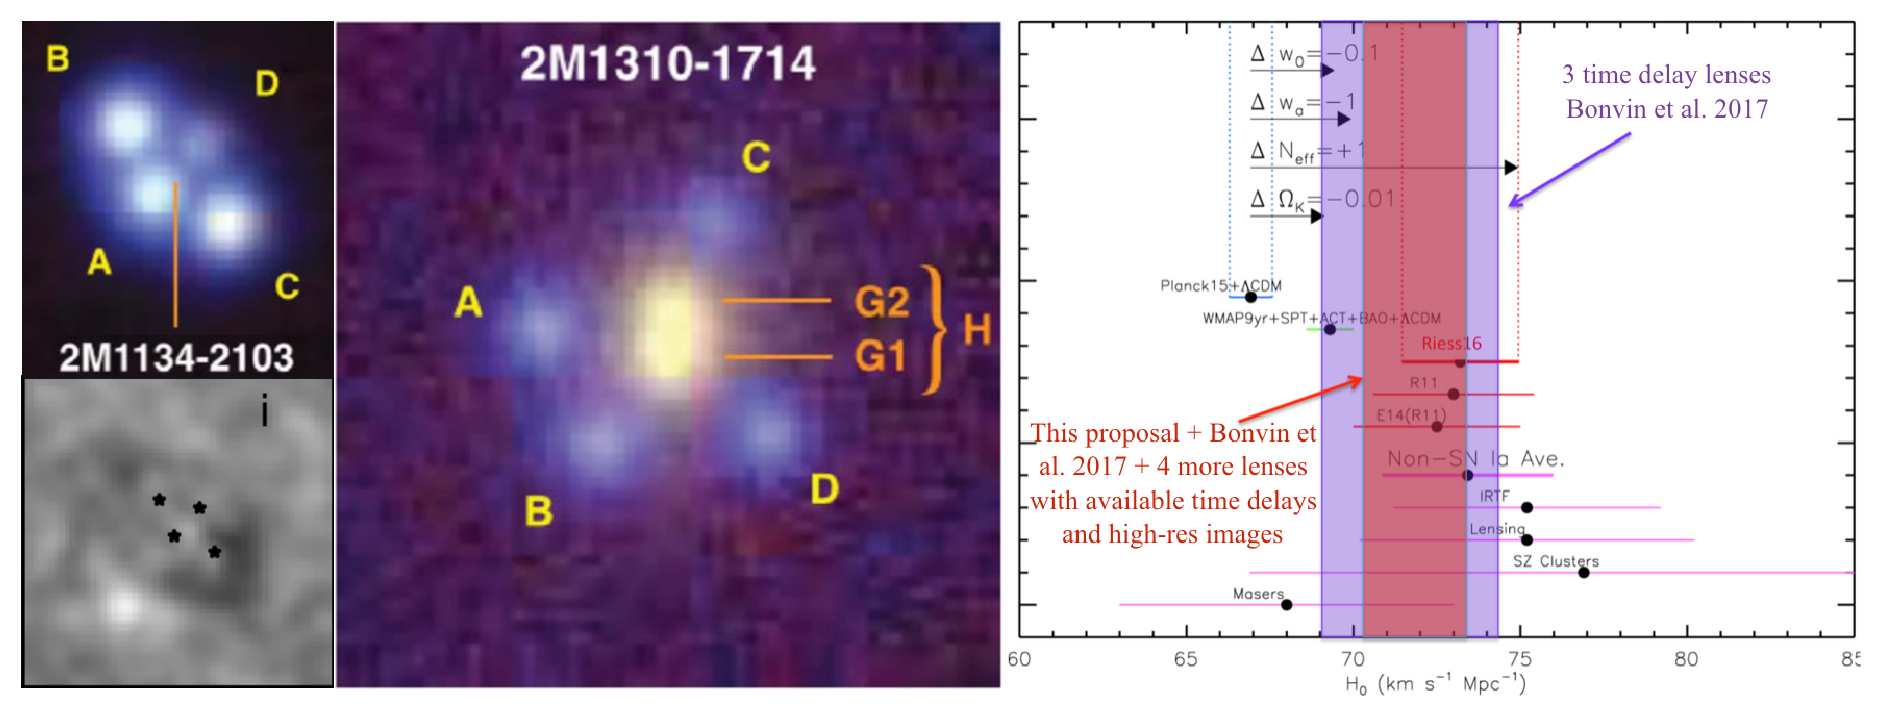
\includegraphics[width=0.95\hsize]{figure.eps}
\end{minipage}
Fig. 1: {\it Top left:} Tension between measurements of $H_{0}$ from different probes in a $\Lambda$CDM cosmology. The {\it Planck} measurement is in tension with the local distance ladder (Riess et al. 2016). The tension could be due to systematic errors in the measurements, or be indicative of new physics (the effects in changing key cosmological parameters are shown as black arrows). Our measurements from three time delay lenses (blue shaded area) is independent of both and can provide vital information if the precision can be further improved. With this proposal, we aim to characterize the mass distribution along the line of sight and constrain $\kappa_\mathrm{ext}$, to get to 2\% precision on $H_{0}$ (red shaded area) from a sample of nine lenses in total. Figure adapted from Riess et al. (2016).
  
{\bf References.} Bolton A.~S., et al., 2008, ApJ, 682, 964-984 $\diamond$ Bonvin V., et al., 2017, MNRAS, 465, 4914 $\diamond$ Courbin, F., et al., A\&A, 516, L12, 2012 $\diamond$ Courbin, F., et al., A\&A, 540, A36, 2012 $\diamond$ Ding X., et al., 2017, MNRAS, 472, 90 $\diamond$ Cen R., et al., 2017, MNRAS, 467, L26 $\diamond$ Gultekin, K. et al., 2009, ApJ, 698, 198 $\diamond$ Guyon et al., 2006, ApJS, 166, 89 $\diamond$ Koopmans et al., 2009, ApJ, 703, L51$\diamond$ Lucey J.~R., et al., MNRAS, 2018 $\diamond$ Meyer R.~A., et al., 2017, arXiv:1711.01184 $\diamond$ More A., et al., 2016, MNRAS, 456, 1595 $\diamond$ Sonnenfeld A., et al., 2018, PASJ, 70, S29 $\diamond$ Oguri M., et al., MNRAS, 439, 2494 $\diamond$ Peng, C., et al., 2007, ApJ, 671, 1098 $\diamond$ Peterson B.~M., 2014, SSRv, 183, 253 $\diamond$ Rusu C.~E., et al., 2016, MNRAS, 458, 2 $\diamond$ Shen et al., 2013, ApJ, 778, 98 $\diamond$ Wong K.~C., et al., 2017, MNRAS, 465, 4895.
Bell \& de Jong 2001, ApJ, 550, 212
$\diamond$ Bonvin et al. 2016, MNRAS submitted (arXiv:1607,01790)
$\diamond$ Collett et al. 2013, MNRAS, 432, 679
$\diamond$ Collett \& Cunnington 2016, MNRAS, 462, 3255
$\diamond$ Courbin et al. 2011, A\&A, 536, 53
%$\diamond$ Eisenstein et al. 2005, ApJ, 633, 560
$\diamond$ Fassnacht et al. 2011, MNRAS, 410, 2167
%$\diamond$ Freedman et al. 2001, ApJ, 553, 47
$\diamond$ Greene et al. 2013, ApJ, 768, 39
$\diamond$ Hilbert et al. 2007, MNRAS, 382, 121
$\diamond$ Hojjati et al. 2013, PhRvD, 87, 123512
$\diamond$ Hu 2005, ASPC, 339, 215
%$\diamond$ Komatsu et al. 2009, ApJS, 180, 330
%$\diamond$ Komatsu et al. 2011, ApJS, 192, 18
$\diamond$ Linder 2011, PhRvD, 84, 123529
$\diamond$ McCully et al. 2016, ApJ submitted (arXiv:1601.05417)
$\diamond$ Perlmutter et al. 1999, ApJ, 517, 565
$\diamond$ Planck Collaboration 2013, A\&A, submitted (arXiv:1303.5076)
$\diamond$ Refsdal 1964, MNRAS, 128, 307
$\diamond$ Riess et al. 1998, AJ, 116, 1009
$\diamond$ Riess et al. 2016, ApJ, 826, 56
$\diamond$ Rusu et al. 2016, MNRAS submitted (arXiv:1607.01047)
$\diamond$ Sekiguchi et al. 2010, JCAP, 3, 15
$\diamond$ Sluse et al. 2016, MNRAS submitted (arXiv:1607.00382)
%$\diamond$ Spergel et al. 2003, ApJS, 148, 175
$\diamond$ Suyu et al. 2009, ApJ, 691, 277
$\diamond$ Suyu et al. 2010, ApJ, 711, 201
$\diamond$ Suyu et al. 2013, ApJ, 766, 70
$\diamond$ Suyu et al. 2014, ApJ, 788, 35
$\diamond$ Suyu et al. 2016, MNRAS submitted (arXiv:1607.00017)
$\diamond$ Tewes et al. 2013a, A\&A, 533, 120
$\diamond$ Tewes et al. 2013b, A\&A, 556, 22
$\diamond$ Treu \& Koopmans 2002, MNRAS, 337, 6
%$\diamond$ Weinberg et al. 2013, PhR, 530, 87
$\diamond$ Wong et al. 2011, ApJ 726, 84
$\diamond$ Wong et al. 2016, MNRAS submitted (arXiv:1607.01403)

\end{document}
